\subsection{Amplitude}
	The Amplitude $ \mathcal{A} $ is a factor which defines the starting volume of a sine wave. It can only take values between 0 and 1.
	\begin{equation}\label{AmplitudeRef}
		\mathcal{A}\subset\R, \quad \mathcal{A}=[0, 1]
	\end{equation}

\subsection{Decay function}
	The decay $ \gamma $ is a linear or exponential function which defines how fast a sine wave will decay over time. With $ x,m,b\in\R $
	\begin{eqnarray}\label{DecayRef}
		\gamma(x)&=&m*(-x)+b\nonumber\\
		\gamma(x)&=&e^{f(x)}
	\end{eqnarray}
	
\subsection{Harmonic Series}
	A harmonic series is a list of frequencies which are contained in a note. Each frequency is a multiple of the base reference but they don't have to be a standard tone step.$ \Nn $
	\begin{eqnarray}
		&\exists n\in\N, F_B=F(n)&\\
		&F_{B_i}:=F_B*i, \quad \forall i\in\N&\\
		&&\\
		&\exists m\in\N, m>n, F_{B_i}=F(m) \Leftrightarrow 12|m-n&
	\end{eqnarray}
	\begin{eqnarray}
		F_{B_i}
		&=&F_B*i\\
		&=&F(n)*i\\
		&=&(f_0*(\sqrt[12]{2})^n)*i\\
		&=&(f_0*(\sqrt[12]{2})^{m-q})*i \qquad q\in\N\\
		&=&(f_0*(\sqrt[12]{2})^m*(\sqrt[12]{2})^{-q})*i \qquad 12|q\\
		&=&(f_0*(\sqrt[12]{2})^m*2^{p})*i \qquad p\in\N, p=\frac{q}{p}\\
	\end{eqnarray}
	\begin{center}
		\begin{tabular}{|ccccccccc|}
			\cline{1-2}
			First octave & $ C_0 $ & \multicolumn{0}{|}{}\\
			\cline{1-3}
			Second octave & $ C_1 $ & $ G_1 $ & \multicolumn{0}{|}{}\\
			\cline{1-5}
			Third octave & $ C_2$ & $E_2$ & $G_2$ & $\approx Bb_2 $&\multicolumn{0}{|}{}\\
			\hline
			Forth octave & $ C_3 $&$ D_3 $&$ E_3 $&$ \approx F_3 $&$ G_3 $&$ \approx Ab_3 $&$ \approx Bb_3 $&$ B_3 $\\
			\hline\hline
			\multicolumn{9}{|c|}{Example for base $ C_0 $}\\
			\hline
		\end{tabular}
	\end{center}

\subsection{Frequency calculation}
	$ n\in\Z $\\
	$ f_0=440 $Hz
	Octave:
	\begin{equation*}
		f_n=f_0*2^n
	\end{equation*}
		$ m\in\Z $
		12 half tone steps per octave
	\begin{equation}
		f_m=f_0*(\sqrt[12]{2})^m
	\end{equation}
	\begin{center}
		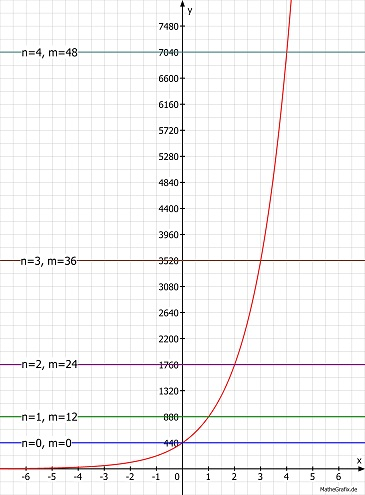
\includegraphics[scale=0.1]{img/frequencyFunction.jpg}
	\end{center}